\section{Module 4. Non-stationary noise filtering 1}

The unit tests was implemented to check how the programme behaves in different conditions. The few tests

\begin{itemize}

	\item \textbf{Test\_empty\_input\_data} - test checks how the code behave in case receiving empty dataset,
	\item \textbf{Test\_incorrect\_input\_data} - test checks how the code behave, when incorrect data is passed to the function,
	\item \textbf{Test\_size\_input\_data} - test checks if the size of data is changed on the output of code,
	\item \textbf{Test\_none\_noise\_map} - if code received empty data of noise maps, the function should rise an error,
	\item \textbf{Test\_LMMSE\_function\_changes} - test checks if the input data was changed in the LMMSE-filter function.

\end{itemize}

The results of tests were as it was expected and code behaves in correct way. To check working of programme implement a demo for code. The results for different images are shown below. The results show one more time that the most correct size of neighbourhood is 6. The images after LMMSE filtration are not perfectly filtered. Brain is sometimes blurred and the contour of brains was filtered worse than other parts. The smaller size window than 4 shows the worst result of filtration. 

\begin{figure}[H]
\centering{}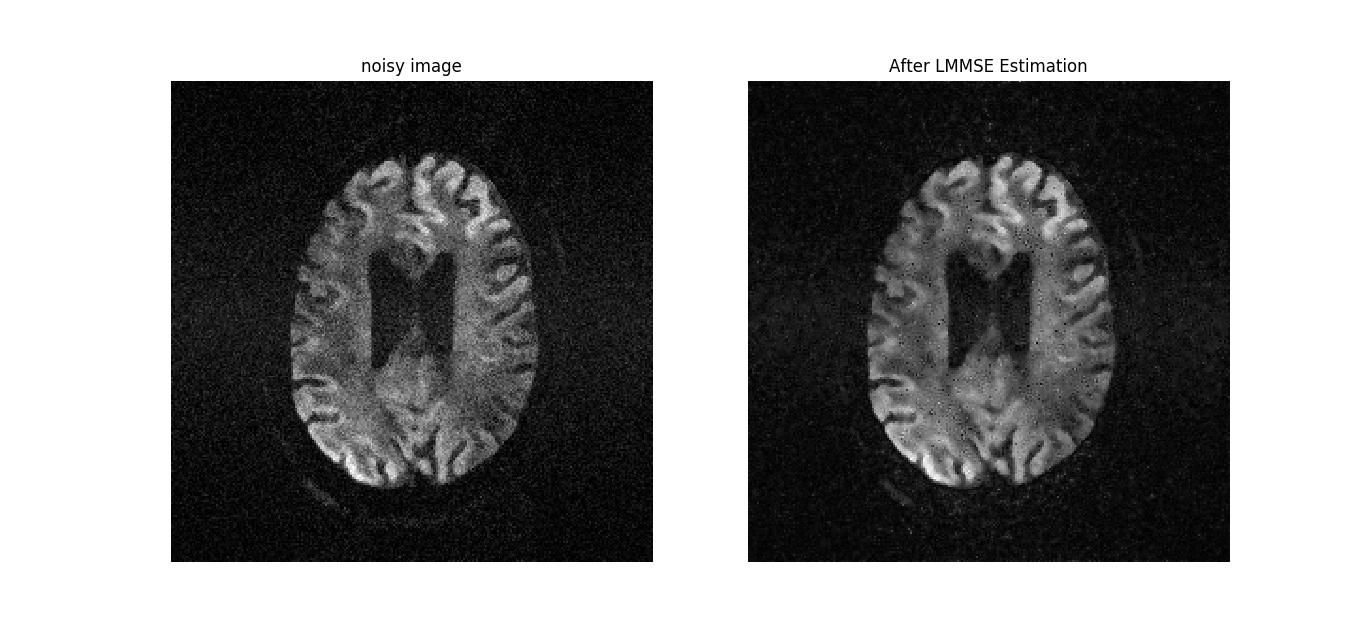
\includegraphics[scale=0.5]{figures/Module_4/diff3}\caption{Results of LMMSE estimation with size window = 3 for diffusion data} \label{fig:figures/Module_4/diff3}
\end{figure}

\begin{figure}[H]
\centering{}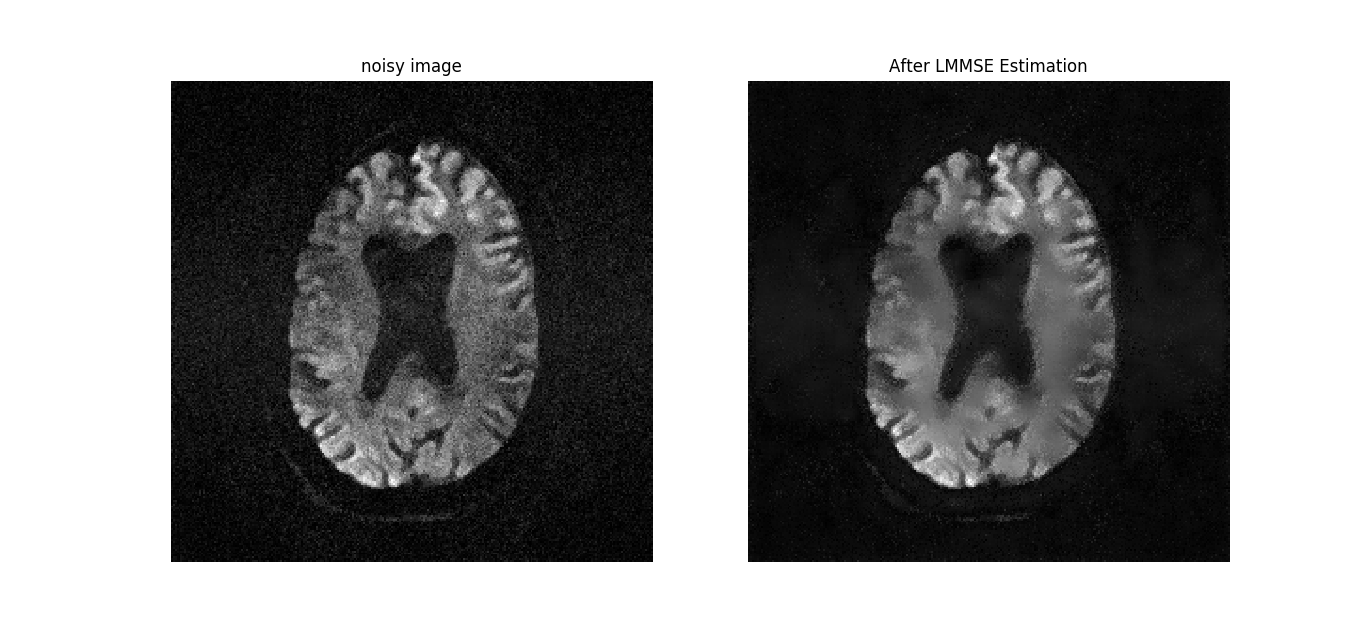
\includegraphics[scale=0.5]{figures/Module_4/diff10}\caption{Results of LMMSE estimation with size window = 10 for diffusion data} \label{fig:figures/Module_4/diff10}
\end{figure}

\begin{figure}[H]
\centering{}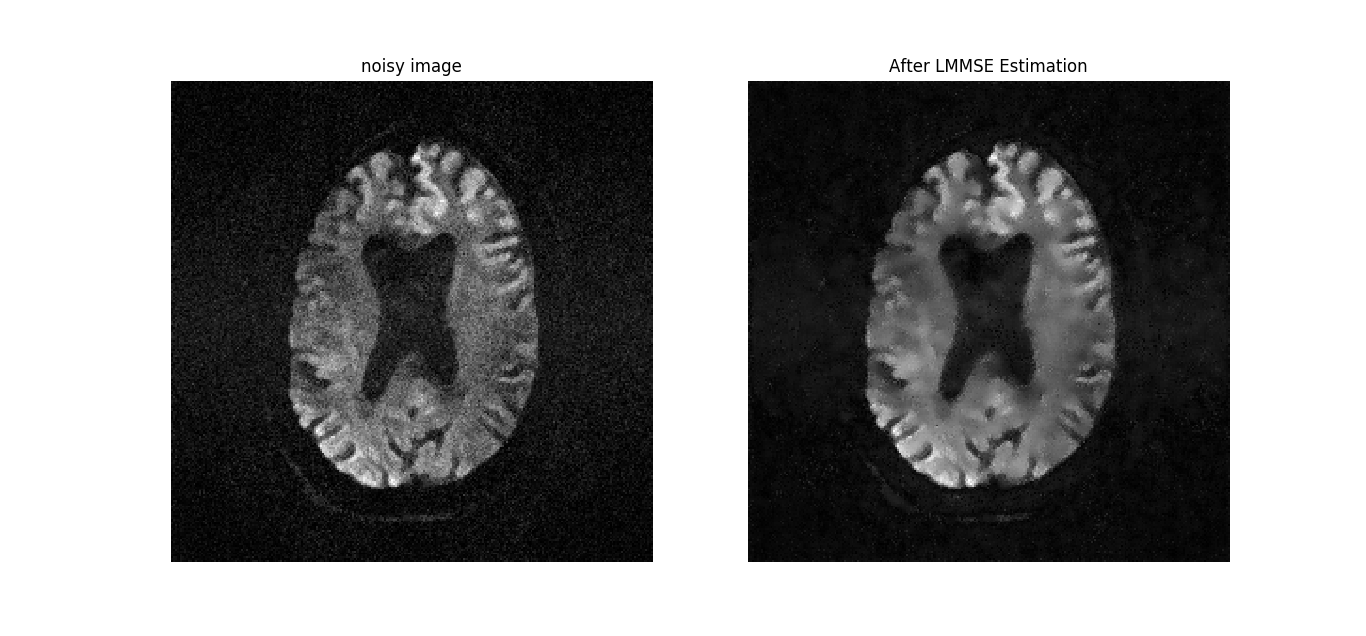
\includegraphics[scale=0.5]{figures/Module_4/LMMSE_dif2}\caption{Results of LMMSE estimation with size window = 6 for diffusion data} \label{fig:figures/Module_4/LMMSE_dif2}
\end{figure}

\begin{figure}[H]
\centering{}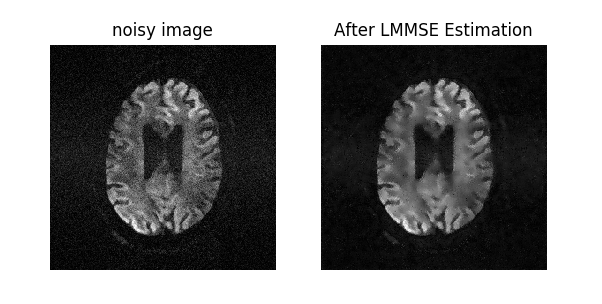
\includegraphics[scale=0.7]{figures/Module_4/LMMSE_dif1}\caption{Results of LMMSE estimation with size window = 6 for diffusion data} \label{fig:figures/Module_4/LMMSE_dif1}
\end{figure}